% Very simple template for lab reports. Most common packages are already included.
\documentclass[a4paper, 10pt]{article}
\usepackage[utf8]{inputenc} % Change according your file encoding
\usepackage{graphicx}
\usepackage{url}
\usepackage{listings}
\usepackage{xcolor}

\definecolor{mygray}{rgb}{0.5,0.5,0.5}

\lstset{
    basicstyle=\footnotesize,
    language=erlang,
    frame=single,
    numbers=left,
    numberstyle=\tiny\color{mygray},
    breaklines=true,
}

%opening
\title{Chordy: a Distributed Hash Table}
\author{Antonios Kouzoupis $<$antkou$@$kth.se$>$}
\date{\today{}}

\begin{document}

\maketitle

\section{Introduction}

In this assignment we have implemented \emph{Chordy}, a Distributed Hash Table
following the \emph{Chord} protocol scheme. Our goal is to build a structured
network of nodes where each node will store only data it is responsible for
(DHT). Each node will be assigned with a random key identifier. Storage will
store \emph{\{key, value\}} data where key is also a random identifier and
data can be anything. Of course data are there for a reason, to be looked up, so
nodes can also look-up for them given their unique identifier.

After the growth of the Internet millions of computers and users required to
had access to shared resources stored in different spots. A key problem that
had to be answered was the way different data should be stored in a distributed system
of computers in order to access them in a workload balanced way and to ensure
availability. Peer-to-peer systems, like Distributed Hash Tables, provided a way
of efficient routing in the network and data replication for availability. Also
exploiting the benefits of consistent hashing they provide load balance to the
system.

\section{Main problems and solutions}

In this assignment, I believe that the most difficult problem was to obtain a
solid understanding of the Chord-like scheme. How a node behaves when it
initially joins the network, finding predecessors and successors and how the
network stabilizes itself. Fortunately that was not hard for me since my
bachelor thesis was based on the \emph{Chord} protocol. Again the majority of
code was given \textbf{but} the pieces we had to fill were not trivial at all.
We have divided the implementation of \emph{Chordy} in two stages, the first one
was to build a working ring and the second one for the ring to be able to to
store and look-up data.

\subsection{The Fellowship of the Ring}

For the first version of our system (node1) first I had to write a random key
generator. So I seed the \texttt{random} module with the current time and
generated a random identifier. The second function of the \emph{key} module was
to identify if a number is between two others. Piece of cake at first though but
a little bit tricky on second. It is trivial to tell whether 4 is between 2 and
5 but not if 4 is between 5 and 2 in a ring structure.

Supposedly, nodes
with ID 5 and 2 are connected to each other (5 successor is 2 and vice versa)
and a node with ID 4 wants to join the network bootstrapping from node with ID 2.
Node 4 will assign 2 as its successor. At some designated interval, Node 2 will
run the \texttt{stabilize} function. First it will \texttt{request} its
successor to send him the successor's predecessor. Then Node 4 will run the
\texttt{stabilize} function. If its successor (Node 2) predecessor (Node 5) is
null it is notified of our existence and we assign it as our successor (this is
not our case in our example). If our successor's predecessor is ourself, then no
trouble, we keep things like this (not our case). If our successor's predecessor
is himself then we also inform it of our existence (not our case either).
Finally, if it someone we do not know, then we check if its ID (5) is between
ours (4) and our successor's (2). Because it is a ring structure, number 5 is
between 4 and 2. In that case we send a \texttt{request} message to Node 5
repeating that procedure and we set it as our new successor. When a node is
notified by a new node, it checks whether that new node's key identifier is
between it's predecessor's key and itself's. If it is, then sets as its new
predecessor that new node, else things do not change.

\subsection{Storage}

In our second version of \emph{Chordy} (node2), I implemented the storage
feature. It was easier than the first part since now we have a working overlay
network. The main idea behind who is responsible for a \emph{\{key, value\}} pair is
the same as before. If the message's key is between our predecessor's key and
ours we store it, otherwise we forward the message to our successor. The same
goes for the look-up of a key. What is worth mentioning is that whenever a
new node joins the network, with a way similar to above, our successor provide
as with the keys we are now responsible for and discharge itself.

\section{Evaluation}

For the evaluation process I wrote a simple test case which takes as arguments
the module that we want to use, node1 or node2 and the number of nodes to spawn.
Also I have added an extra message handler in node2 module (\texttt{status}) which shows the
predecessor, the successor and the storage of nodes. 

Our first test will be to prove that ring is indeed created and nodes are
connected. So we spawn some nodes and send a \texttt{probe}. The output proves
that probe passed from every node, so the network is stabilized. In order to
double check I sent a \texttt{status} message to all of them to print their
predecessors and successors.

In Figure \ref{fig:probe_tt} we see the time a probe takes to travel all around
the network. Note that if I set the stabilize interval quite high, the network
takes more time stabilize. While I was testing the interval time, in high
values, some nodes were not listed in the probe output since they were not
integrated in the ring.

\begin{figure}[h!]
\begin{center}
    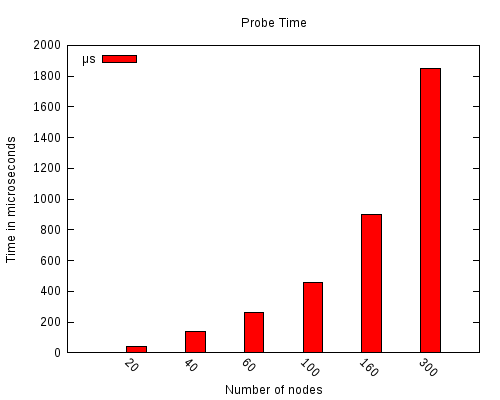
\includegraphics[scale=0.4]{histograms/probe_tt.png}
    \caption{Probe time in $\mu$s}
    \label{fig:probe_tt}
\end{center}
\end{figure}

For measuring the performance of our DHT I extended my first test case with a
function which takes as arguments a node to contact and the number of messages
to add. After sending the \texttt{add} message, is waiting for the response
\texttt{\{QRef, ok\}} and finally it prints the time it took and returns the
list keys in order to use them for look-up. The look-up function has almost the
same functionality. It gets the keys, sends the \texttt{lookup} message and waits
for the response. Then it prints the time it took for the lookup. In Figures
\ref{fig:add} and \ref{fig:lookup} is illustrated the time needed to add and
lookup
various number of items on a network of 10 nodes. We can see that adding items
in the network with random key identifiers (both for nodes ID and key in items)
is much more faster than with sequential identifiers. This is happening because
in the first occasion keys with ID bigger than 10 are stored in the same node
which maybe ``far'' from the bootstrap node. Whereas in the random IDs, the keys
are almost evenly distributed among the nodes.

On the contrary, when we do look-up operations, the time is almost the same
(not). The experiment was setup to be like this, in order to emphasize the
difference in distribution between the two approaches. In sequential keys, the
look-up is made through the first node of the ring which has the most of the
keys. When I did the lookup through another node, the time was much more higher.
But in the case of random generated keys, items are evenly distributed in the
ring so the look-up time is almost the same regardless of which node we use for
the operation.

The final part of my evaluation was to show that when a node joins the network,
it takes responsibility for some keys. So I used sequential IDs and I initially
added nodes 1, 2, 5 and keys 1, 2, 3, 4, 5. Items with key 1 and 2 where added
to nodes 1 and 2 respectively and items with key 3, 4, 5 to node 5. After that,
node with ID 4 joined the network. Using the \texttt{status} message handling, I
examined the storage for every node. Nodes 1 and 2 had no changes of course, but
now keys 3 and 4 from node 5 where transferred to node 4, which is what we
expected. Now data are more evenly distributed making add and lookup operations
in the ring more efficient.

In another scenario, I have spawned only one node and four clients are asking to
add 1000 items each. The total time for add is 684400 $\mu$s and for look-up is
159200 $\mu$s. When I add three more nodes the performance is more or less the
same for addition (590000 $\mu$s) and for look-up is worse 431946 $\mu$s. The more
nodes I added the more time it took for the operations to performed. For
example, when I spawned 1000 nodes, time for addition was 1605610 $\mu$s and for
look-up 1083405 $\mu$s. Probably one have to find the golden ratio between the
number of nodes and the amount of data that is expected for the system to store.
Also we have to make a bargain between performance and availability, two factors
that usually cannot coexist.

\begin{figure}[h!]
\begin{center}
    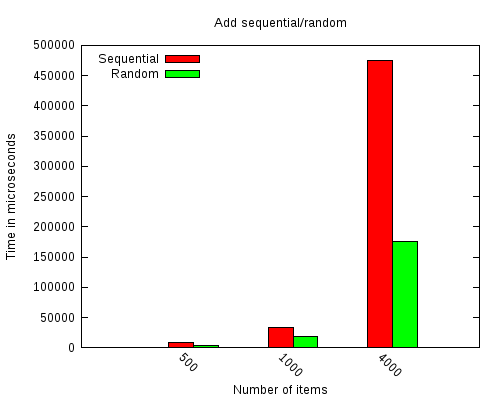
\includegraphics[scale=0.4]{histograms/add_seq_rnd.png}
    \caption{Adding time in $\mu$s for sequential and random IDs}
    \label{fig:add}
\end{center}
\end{figure}

\begin{figure}[h!]
\begin{center}
    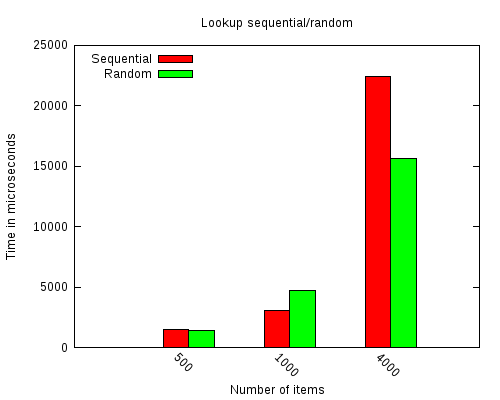
\includegraphics[scale=0.4]{histograms/lookup_seq_rnd.png}
    \caption{Lookup time in $\mu$s for sequential and random IDs}
    \label{fig:lookup}
\end{center}
\end{figure}
\section{Conclusions}

In this last assignment we have implemented \emph{Chordy}, a Distributed Hash
Table. We can form a ring, add content to the nodes and look-up for data.
Unfortunately I did not have enough time to continue with the extra sections of
handling failures and replication. It is quite easy to maintain a distributed
storage when you are dealing with immutable objects since you do not have to
worry for consistency but when it comes to mutable it is tricky.

\end{document}
